%!TEX root = ../Fachentwurf.tex

\chapter{Einleitung}
Ziel dieses Dokuments ist es, einen tiefer gehenden Überblick über den internen Ablauf der zu entwickelnden Software zu bieten. Es werden zuerst die wichtigsten Funktionen einzeln beschrieben, wobei Sequenzdiagramme zu Hilfe genommen werden. Danach wird die Datenverwaltung näher beleuchtet. \\

\begin{figure}[h]
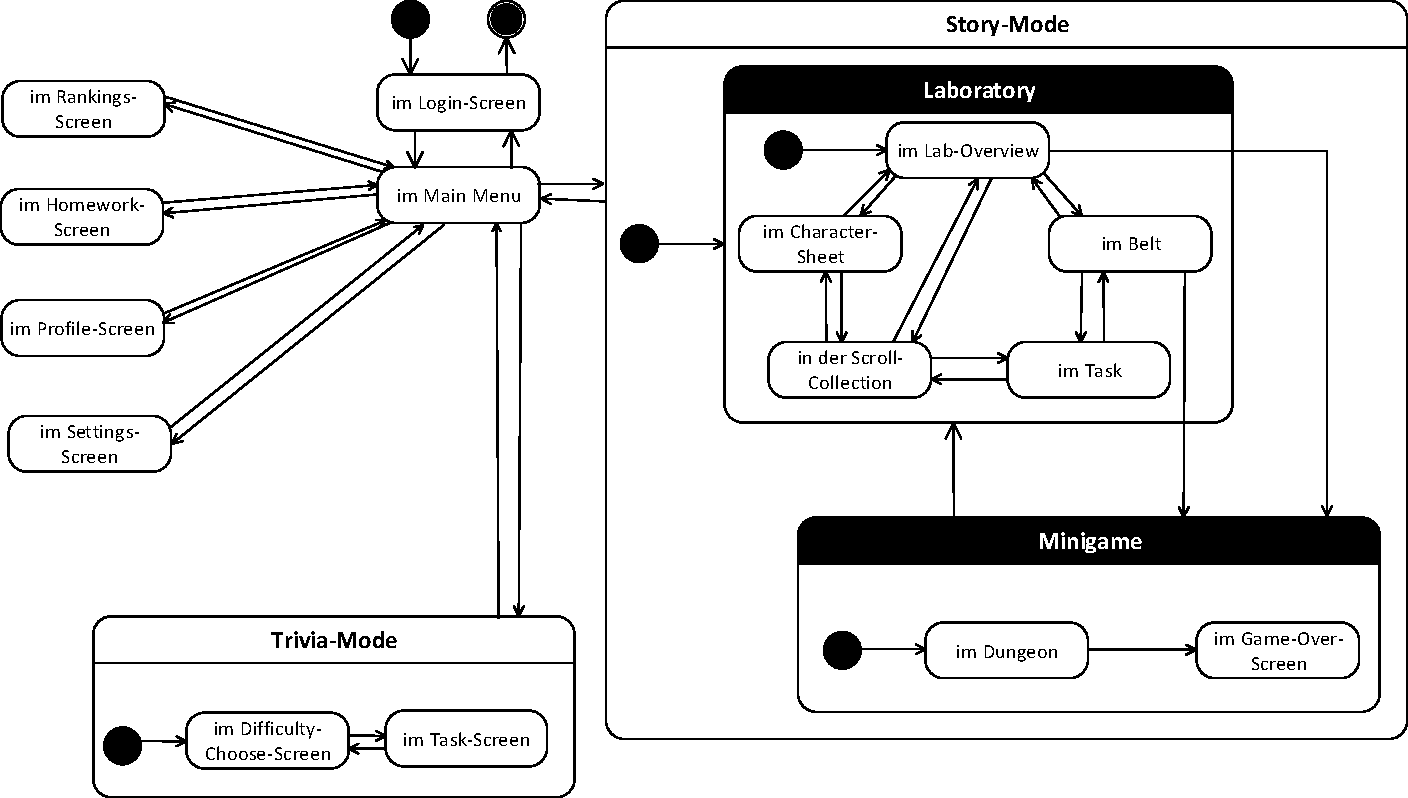
\includegraphics[width=1.0\textwidth]{figures/statechart_game.pdf}
\caption{Zustandsdiagramm zum oberflächlichen Spielablauf}
\label{sequence}
\end{figure}


Um eine Verständnisgrundlage zu schaffen ist in Abbildung 1.1 der allgemeine Men\"uf\"uhrung in einem Aktivit\"atsdiadramm dargestellt. 


Nach dem Einloggen gelangt man in das Main Menu. Von dort aus gelangt man in die drei Spielmodi (Story, Trivia, Homework), die Einstellungen, das Profil und in die Ranglisten.

Der Story Mode hat wiederum eine eigene Übersicht, Laboratory genannt. Von hier aus kann der User sich seine aktuellen Playerstatistiken im Charakter Sheet ansehen, kann sich in der Scrollcollection um die Herstellung von Potions und Enchantments k\"ummern, diese danach in seinen Belt einf\"ugen um sich im Anschluss dem Minispiel zu widmen. Im Minispiel werden dem User verschiedene Hindernisse vorgesetzt, die es zu überwinden gilt. Scheitert der User, so gelangt er in den Game Over Screen, in dem ihm angezeigt wird wie viele Lofi-Coins (die Spiel-Währung) und welche Scrolls er in dieser Runde eingesammelt hat. Nach Bestätigung befindet sich der User zurück im Laboratory.

Der Trivia-Mode stellt einen SQL-Trainer dar. Entscheidet der User sich dafür diesem zu verwenden, gelangt er in einen Screen in dem er sich für einen Schwierigkeitsgrad entscheiden muss. Hat der User dies getan, erhält er eine, dem ausgewählten Schwierigkeitsgrad entsprechende, Aufgabe und kann diese lösen.

Der Homework-Mode funktioniert genauso wie der Trivia-Mode, lediglich die Auswahl des Schwierigkeitsgrads entf\"allt in diesem Fall.

In den Rankings werden die Spieler nach verschiedenen Kriterien in Ranglisten sortiert. Darüber ist es auch möglich durch die Eingabe des Usernamens nach anderen Spielern zu suchen und sich deren Profile anzeigen zu lassen.
Das eigene Profil ist über das Main Menu zu erreichen und einsehbar. Selbiges gilt für die Spieleinstellungen.  



\section{Projektdetails}

Die Anzahl an Lofi-Coins, sowie die Anzahl an Scroll die der User pro Tag einsammeln kann, werden beschr\"ankt.
Dies soll verhindern, dass der User nicht den Fokus, des \"Ubens von SQL-Statements, verliert. Auf der anderen Seite jedoch, soll so der Spieler zum Wiederkommen
animiert werden.

Desweiteren wurde im Pflichtenheft erwähnt, dass Spieler sich durch Aufgabenerstellung ins Spiel mit einbringen können. Um dabei jedoch eine gewisse Qualität zu gewährleisten zu k\"onnen, wird es nur beförderten Nutzern möglich sein, eigene Aufgaben zu erstellen. Wie ein User befördert wird, wird über die Spielzeit oder über Leistungen im Spiel geregelt.  

%Besonders interessante oder komplizierte Sachverhalte sollen hier noch weiter vertieft werden.
 %Auch hier sollen Aktivitätsdiagrame und Statecharts verwendet werden.

%Beispiele:
%\begin{itemize}
%\item Bei einem Spiel könnten komplizierte Regeln dargestellt werden.
%\item In einen Web-System könnte bestimmte Workflows als Aktivitätsdiagramm dargestellt werden.
%\end{itemize}

%Es kann pro Sachverhalt ein Abschnitt hinzugefügt werden.

